\capitulo{5}{Conclusiones}


\section{Resumen de resultados}
Los resultados obtenidos han sido satisfactorios, se ha cumplido el objetivo principal de este Trabajo de Fin de Grado, se ha logrado simular la funcionalidad de una válvula ventriculoperitoneal. Esta válvula es un dispositivo médico utilizado para derivar el exceso de líquido cefalorraquídeo (LCR) desde el sistema ventricular del cerebro hasta el peritoneo (para más información consultar la sección de \textit{Conceptos teóricos}), lo que ayuda a aliviar la presión intracraneal elevada. En este proyecto, se ha replicado este proceso mediante un sistema compuesto por un relé, un sensor de presión, y una mini bomba, verificando que todos los componentes funcionaban de forma correcta antes de montar el circuito completo. En el \textit{Anexo G} podemos encontrar las pruebas realizadas con el relé y el sensor, junto con el código necesario para su ejecución.


El montaje consiste en un recipiente que representa el cráneo, en cuyo interior podemos encontrar el sensor y la mini bomba. Al añadir agua a este recipiente, la presión aumenta, y este cambio será detectado por el sensor. Cuando la presión alcanza un umbral predeterminado, el relé activará la mini bomba, permitiendo el paso del líquido a otro recipiente, que simulará el peritoneo. En la Figura \ref{fig:proyect-realiad} podemos observar el montaje.

\begin{figure}[h]
    \centering
    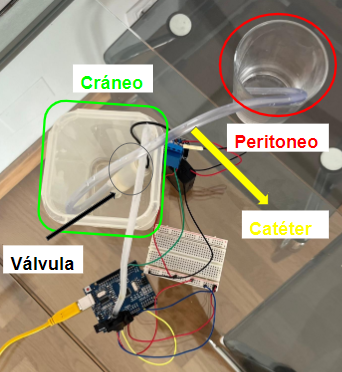
\includegraphics[width=0.7\textwidth]{img/proyect-realidad.PNG}
    \caption{Identificación de los componentes con el cuerpo humano. Imagen propia.}
    \label{fig:proyect-realiad}
\end{figure}

\newpage

\section{Discusión}
Como he mencionado anteriormente, los resultados han sido los esperados. No obstante, cabe destacar algunos detalles. En el código, el valor de presión predeterminado para que se active el relé es de 4 mmHg, y en el cuerpo humano entre 5-15 mmHg se consideran valores normales, no se requiere de atención médica hasta que no se alcancen los 20 mmHg. En este trabajo, se ha elegido el valor de 4 mmHg debido al recipiente empleado, se necesitaría un recipiente más alto y grande para lograr presiones de 20 mmHg. El problema radica en la limitación presentada por los cables. El cable de la mini bomba es demasiado corto para introducirlo en un recipiente más alto ya que se introduciría también el relé al que está conectado. Aún así el programa sería el mismo, salvo el valor de presión preestablecido. 

\section{Aspectos relevantes}

A lo largo de la elaboración de este proyecto se pueden destacar varios aspectos relevantes. 

En primer lugar, la identificación de carencias en el campo de la neurocirugía, la falta de dispositivos que empleen la telemetría\footnote{La telemetría es una tecnología de medición remota que permite recoger, procesar y transmitir la información de un dispositivo electrónico a otro\cite{telemetria}} para dar solución a diferentes problemas dentro de este área. A través de plataformas como Arduino y la selección de diferentes componentes electrónicos, se ha simulado la funcionalidad de una válvula de derivación, implementando un sistema automatizado que ajuste su apertura en base a las lecturas del sensor. Este sistema de regulación brinda una solución más precisa y personalizada, ya que la válvula está controlada en todo momento, ajustándose a las necesidades que requiera cada paciente. 

Además, se plantea el desarrollo de una aplicación móvil para conseguir monitorizar a los pacientes y controlar el dispositivo de una forma no invasiva, lo cual se convierte en un aspecto clave para lograr un manejo eficiente del dispositivo. Uno de los objetivos principales de este proyecto radica en la importancia de la medicina personalizada\footnote{La medicina personalizada busca el tratamiento adecuado a cada paciente sobre la base del diagnóstico preciso, las terapias dirigidas y el análisis de los datos \cite{med_per}.} ya que cada persona es diferente y por lo tanto las soluciones deben de estar enfocadas en ceñirse lo máximo posible al perfil de cada paciente. La aplicación permitirá realizar ajustes específicos del dispositivo basándose en las necesidades individuales y consiguiendo así mejorar de forma exponencial los resultados clínicos y la calidad de vida del paciente.

Este proyecto ofrece una base sólida para futuras investigaciones en el campo de la neurocirugía y la tecnología, abriendo nuevas puertas a diferentes soluciones y mejoras en el tratamiento de la hidrocefalia. Combina conocimientos de diferentes campos tales como la neurocirugía, ingeniería de la salud y desarrollo de software entre otros, mostrando la importancia del trabajo conjunto de diferentes áreas para conseguir dar solución a diferentes problemas en el ámbito de la medicina.

En resumen, estos serían los aspectos más relevantes del proyecto:
\begin{enumerate}
    \item Identificación de carencias en la Neurocirugía
    \item Aplicación práctica de la tecnología
    \item Sistema Automatizado
    \item Medicina Personalizada
    \item Base para futuros proyectos
    \item Interdisciplinariedad
\end{enumerate}







